\section{Small Dynamic Subsystem Interface Protocol Architecture}
\label{sec:sdsip}

The Small Dynamic Subsystem Interface Protocol (SDSIP) is, as the name implies, a standardized method of communication
between subsystems. That is, the protocol is not limited to avionics\footnote{Although the focus of its implementation
in this work being on an avionics system}. Its design is meant to focus on generating interfaces to SDSIP compatible
drivers seamless as well as making transmitting and receiving data from other subsystems simple.

The overall operational architecture of SDSIP is represented in \autoref{fig:sdsip-operational-architecture}. SDSIP is
composed of an API\footnote{Much like Vulkan or OpenGL where applications that which to utilize the framework write code
that utilize its functionality} and an application.

\begin{figure*}[ht]
  \begin{center}
    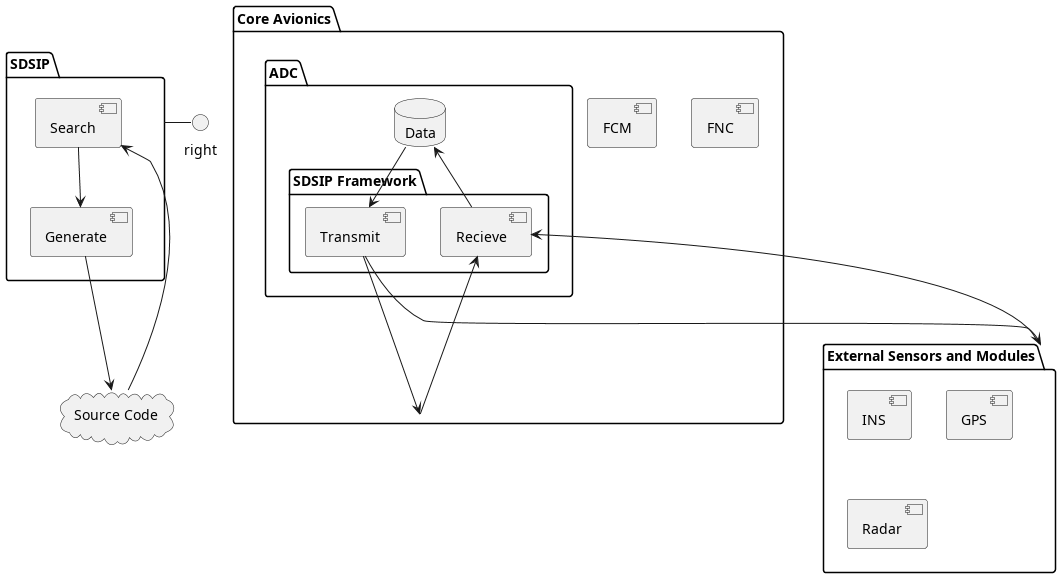
\includegraphics[width=0.90\textwidth]{sdsip-operational-architecture}
  \end{center}
  \caption{}
  \label{fig:sdsip-operational-architecture}
\end{figure*}
